% Evaluation criterion:
%- Language and use of figures
%- Clarity of the problem statement
%- Overall document structure
%- Depth of understanding for the field of computer architecture
%- Depth of understanding of the investigated problem

\section{Introduction}
\label{sec:introduction}
Processor performance has increased more than memory performance,
which has led to what is commonly known as the Memory Gap (see figure~\ref{img:mem_gap}). In order to remedy this, a memory
hierarchy is used to provide the illusion of a very fast and very
large memory (see figure~\ref{img:mem_hier}). 

\begin{figure}[H]
	\centering
	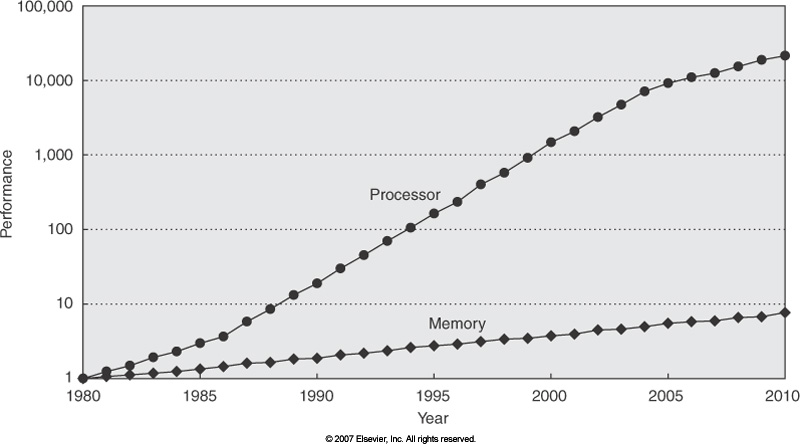
\includegraphics[scale=0.3]{./img/mem_gap}
	\caption{The memory gap}
	\label{img:mem_gap}
\end{figure}

The illusion will only partially hold, however, as the processor is
delayed for the entire main memory access time when memory contents it
needs to access is not present in one of the caches. One technique
which has been introduced in order to leverage this speed discrepancy
by utilising caches more efficiently is prefetching. This technique
attempts to improve the cache hit rate by predicting what memory
addresses the processor will want to access in the near future, and
issuing fetches from the main memory before the processor actually
needs the contents so that the data will reside in cache when the
processor does require it. This is usually accomplished by recording
memory access history and statistics, and using this to make educated
guesses about the future. 
{\bf (references, citations)}

\begin{figure}[H]
	\centering
	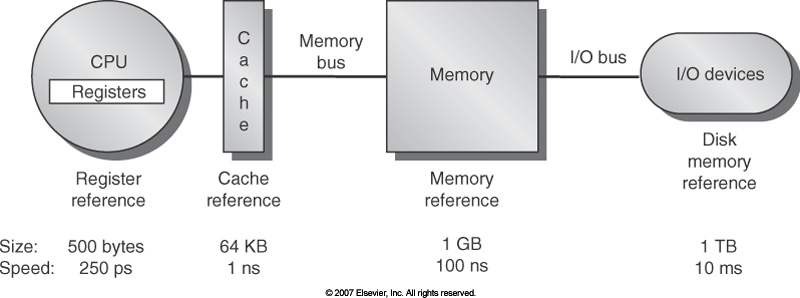
\includegraphics[scale=0.3]{./img/mem_hier}
	\caption{The memory hierarchy}
	\label{img:mem_hier}
\end{figure}

In this paper, we are going to investigate how different kinds of
prefetching strategies affects the efficiency of the prefetcher when
run on several different programs from the SPEC CPU2000 benchmark
suite.  {\bf (references, citations)}
